\documentclass[letterpaper, reqno,11pt]{article}
\usepackage[margin=1.0in]{geometry}
\usepackage{color,latexsym,amsmath,amssymb,graphicx, float}
\usepackage{hyperref}

\hypersetup{
colorlinks=true,
linkcolor=magenta,
filecolor=magenta,
urlcolor=cyan,
}

\graphicspath{ {images/} }

\begin{document}
\pagenumbering{arabic}
\title{PHYS 350 Final Project}
\date{April 11, 2022}
\author{Xander Naumenko, 38198354}
\maketitle

\tableofcontents

\section{Introduction}
 
The goal of this paper is to explore the consequences of alternate physical laws in Lagrangian mechanics, more specifically the consequences of a different expression for gravitational potential. Two body motion is explored for these alternate laws, with an emphasis on contrasting the results with the real world $U\approx\frac{1}{r}$ law. 

\section{Problem Statement}

One fundamental law that yields surprisingly beautiful results is the fact that the gravitational potential goes with $\frac{1}{r}$. But it is interesting to explore how exactly physical systems evolve when this isn't the case. Here we will explore gravitational potentials of the form: 
\[
U_n(r)=-\frac{G_nm_1m_2}{r^{n}}=-\frac{\alpha}{r^{n}}
,\]
where $G_n$ is an arbitrary constant with SI units $\text{N}\cdot \text{m}^{n+1}\cdot \text{kg}^{-2}$. Specifically we will focus on the case of the two body problem and the resultant orbits with these other reciprocal laws. 

\section{Background}

In class we derived up to the expression for effective potential without making reference to the specific (radial dependent) gravitational potential. As this was derived in class the derivation will not be repeated, but for a system of two bodies of mass $ m_1, m_2$, position $\vec r_1, \vec r_2$ and initial conditions, we found that 
\[
\vec r_{cm}=\frac{m_1\vec r_1+m_2\vec r_2}{m_1+m_2}
,\]
\[
\vec r_{rel}=\vec r_2-\vec r_1
,\]
\[
\vec r_{cm}=\vec v_{cm, \text{initial}}t+\vec r_{cm, \text{initial}}
.\]
Thus the only part needed to solve is the relative motion. For convenience $r$ without subscript will be used to represent $|\vec r_{rel}|$. Then we also found that 
 \[
U_{eff}(r)=\frac{l^2}{2\mu r^2}+U(r)
\]
\[
E_{rel}=\frac{\mu\dot r^2}{2}+U_{eff}(r)
\]
where $U_{eff}$ is the effective potential between the bodies, $E_{rel}$ is the relative energy from their relative motion and $l=\left| r_0\times \mu\vec v_0 \right| $. 

\section{Equilibrium Points}

The obvious next step is to find the equilibrium orbit distant, i.e. the point where $\frac{dU_n}{dr}=0$. Here we see the first interesting effect of our alternate potential: for any $n\neq 2$, solving for the equilibrium distance $p$ gives us
\[
\frac{dU_n}{dr}\bigg|_{r=p_n}=-\frac{l^2}{\mu p_n^3}+\frac{n\alpha}{p_n^{n+1}}=0\implies p_n=\left( \frac{l^2}{ n\alpha\mu} \right)^{1 /(2-n)}
\]
which matches $p=\frac{l^2}{\mu\alpha}$ for $n=1$. However, if $n=2$ then this isn't valid since we're dividing by zero, so the $n=2$ case just reduces to
\[
U_{eff}=\left( \frac{l^2}{2\mu}-\alpha \right)\frac{1}{r^2}\equiv \frac{C}{r^2}
.\]
This is missing the characteristic well that the effective potential normally exhibits, which means that depending on the initial conditions, the relative distance will either got to infinity or $0$ depending on whether $C\geq 0$. To get an intuitive feel for how these different potentials behave, they are graphed in figure \ref{fig:U-plots}. 

\begin{figure}[htpb]
    \centering
    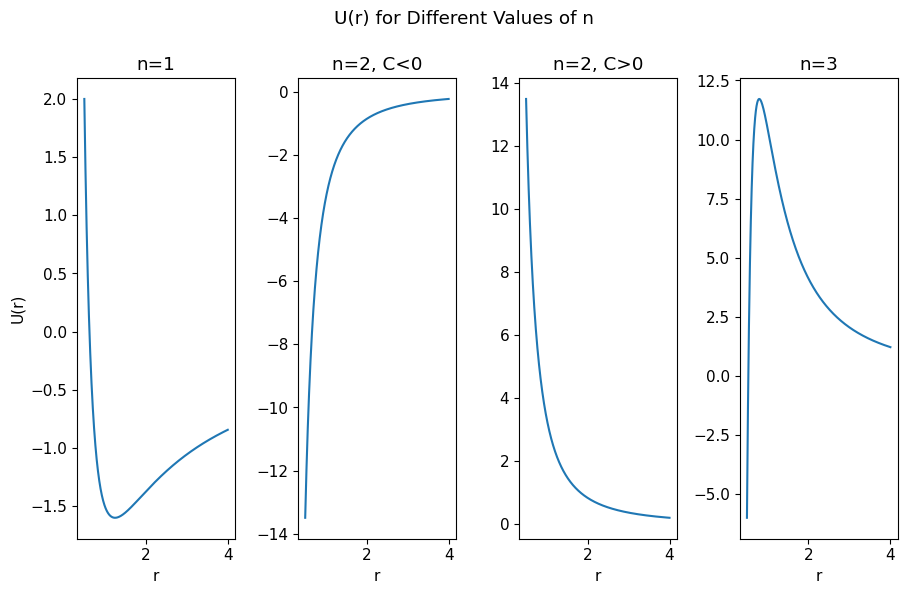
\includegraphics[width=0.8\textwidth]{U-plots}
    \caption{Plots of the shapes of potentials resulting from different values of n. The middle two are both the $n=2$ case, with the left one being with $C>0$ and the other with $C<0$. Note that for $n=1$, there is the characteristic potential well that symbolizes $r=p$. This is not present for $n=2$, but is for $n=3$ except concave down. }
    \label{fig:U-plots}
\end{figure}

Of course this doesn't just apply to integer values of  $n$. Looking at the plots, one might expect that $n<2$ produces stable equilibrium points, while $n>2$ would produce unstable equilibrium points. For this to be the case it needs to be that for $n<2$,  
\[
\frac{d^2U_n}{dr^2}\bigg|_{r=p_n}=\frac{3l^2}{\mu p_n^{4}}-\frac{n(n+1)\alpha}{p_n^{n+2}}>0\implies p_n^{2-n}<\frac{3l^2}{\mu\alpha n (n+1)}
.\]
Plugging in our equation for $p_n$ to this equation gives confirms that 
\[
p_n^{2-n}=\frac{l^2}{n\alpha\mu}< \frac{3}{n+1} \frac{l^2}{n\alpha\mu}  \text{ (for $n<2$)}
\]
as required for $p_n$ to be a stable equilibrium point. In the exact same vein (essentially just switching the directions of inequality), we can show that $n>2$ produces unstable equilibrium: 
\[
\frac{d^2U_n}{dr^2}\bigg|_{r=p_n}=\frac{3l^2}{\mu p_n^{4}}-\frac{n(n+1)\alpha}{p_n^{n+2}}<0\implies p_n^{2-n}>\frac{3l^2}{\mu\alpha n (n+1)}
.\]
Again plugging in the equilibrium point: 
\[
p_n^{2-n}=\frac{l^2}{n\alpha\mu}> \frac{3}{n+1} \frac{l^2}{n\alpha\mu}  \text{ (for $n>2$)}
\]

\section{Trajectory}

Ideally one would like to be able to analytically solve for the trajectory of all of these alternate potentials, similarly to how we did in the $n=1$ case. To go about doing so, note that rearranging $l=\mu r^2\dot\phi$ and combining it with the fact that $E_{rel}=\frac{\mu \dot r^2}{2} +U_{eff}(r)\equiv E$ gives 
\[
d\phi=\frac{l}{\mu r^2}dt=\frac{l}{\mu r^2}\frac{\sqrt{\mu}dr }{\sqrt{ 2(E-U_eff(r))}}\implies\phi=\int \frac{ldr}{r^2\sqrt{2\mu\left( E-U_{eff}(r) \right) } }
.\]
Unfortunately, this integral turns out to be impossible to analytically solve for almost all values of $n$. While it's difficult to show this rigorously, I tried with an integral calculator for a while and no solutions were present. The only exceptions to this were the $n=1$ and $n=2$ case. Then $n=1$ case is of course gravity's actual potential, which we've already solved. The $n=2$ case however is slightly different. For $n=2$ the effective potential is $U_{eff}=\left( \frac{l^2}{2\mu}-\alpha \right)\frac{1}{r^2}\equiv \frac{C}{r^2}$. Thus the integral we are trying to solve is 
\[
\phi=\int \frac{ldr}{r^2\sqrt{2\mu\left( E-C /r^2 \right) } }
.\]
Let $u=\frac{1}{r}$. Then $du=-\frac{1}{r^2} dr$: 
\[
\phi = -\frac{l}{\sqrt{2\mu} }\int \frac{du}{\sqrt{E-Cu^2} }
.\]
For now assume $C\geq0$. Let $u^2=\frac{E}{C}\cos^2 x$. Then $u=\sqrt{\frac{E}{C}}\cos x\implies du=-\sqrt{\frac{E}{C}}\sin x$. Substituting, we get
\[
\phi=-\frac{l}{\sqrt{2\mu} }\int \frac{-\sqrt{\frac{E}{C}}\sin x }{\sqrt{E} \sqrt{1-\cos^2x} }=\frac{l}{\sqrt{2\mu C}}x
.\]
Combining this with the fact that $u=\sqrt{\frac{E}{C}}\cos x=\frac{1}{r}$, we get that
\[
\frac{1}{r}=\sqrt{\frac{E}{C}}\cos\left( \frac{\sqrt{2\mu C}}{l}\phi  \right)  
.\]
We can clean up slightly by expanding $C$ back out in terms of its components and defining $p_2=\sqrt{\frac{C}{E}} $. 
\[
\frac{p_2}{r}=\cos\left( \sqrt{1- \frac{2\mu\alpha}{l^2}} \phi \right) 
.\]
Note that it's very tempting to look at the $\left( \frac{l^2}{\mu\alpha} \right)^{-1} $ in the cosine and try and notice that it happens to be $p_1^{-1}$, and then confuse yourself with the units (inside the square root should have no units, not $m^{-1}$). However $\alpha$ is defined differently in the $n=1$ and $n=2$ case, as $G_1$ and $G_2$ have different units, so the claim of significance for $ p_1$ showing up in the $n=2$ case isn't altogether clear. Instead, define $e_2=\sqrt{1-\frac{2\mu\alpha}{l^2}}  $. Of course both $e_2$ and $p_2$ are defined quite differently here than in the $n=1$ case, but in some sense they both still match the units and functionality of their counterparts. For example $e_2=0$ still produces a circular orbit, as 



\end{document}
